\section{Hormigas}
%\subsection{Metaheur\'istica ACO }
\begin{frame}{Hormigas (OE 1)}
    \centering
    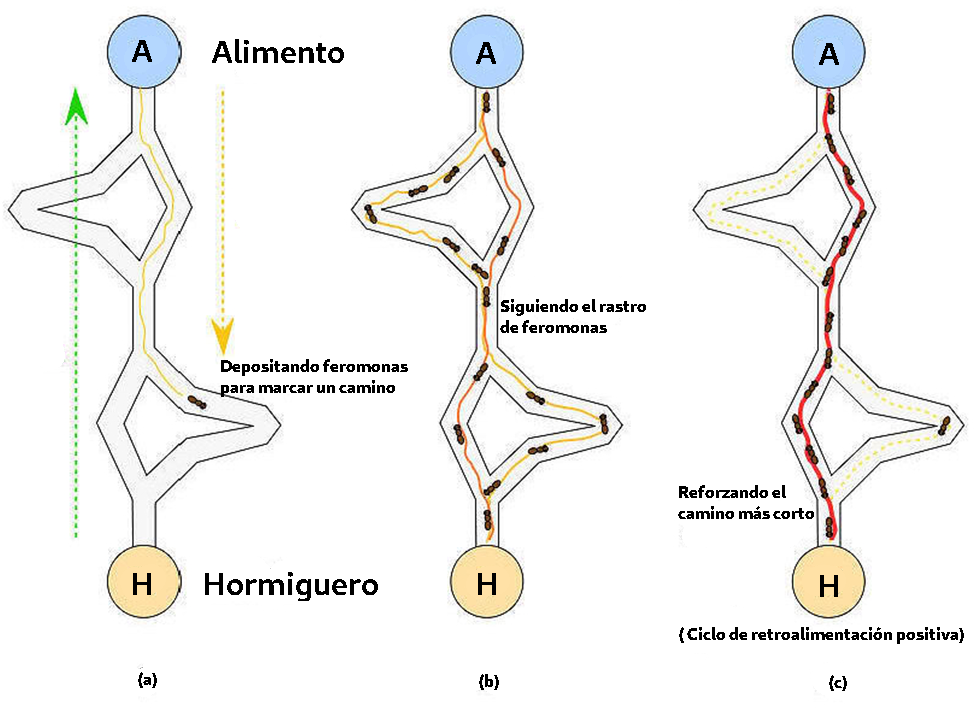
\includegraphics[height=2.5in]{Pictures/ACO-ant.png}
\end{frame}

\note[itemize]{
    \item Como se mencion\'o previamente, uno de los problemas principales al individualizar filamentos es que se desconoce el comienzo y el final de un filamento al comienzo del problema. 
    \item As\'i, resulta natural explorar el comportamiento de las hormigas al buscar alimento como inspiraci\'on para individualizar filamentos. Este comportamiento se puede resumir en las 3 etapas que se muestran en la imagen.
    \item En una primera etapa, a la izquierda de la imagen en la letra {\bf a}, se puede observar que una hormiga que sale del hormiguero recorre un camino aleatorio hasta llegar al alimento. En su retorno, por el mismo camino, deposita feromonas para indicarle a otras hormigas por donde fue su recorrido.
    
    \item Luego, otras hormigas pueden tomar esta informaci\'on en su propio descubrimiento de un camino hacia el alimento, como se observa el la mitad de la imagen, en {\bf b}
    
    \item Finalmente, a la derecha de la imagen, se observa que las hormigas depositan m\'as y m\'as feromonas en el camino m\'as corto entre el hormiguero y el alimento, causando una convergencia sobre un camino \'optimo. Esta convergencia es lo que se define como el ciclo de reforzamiento positivo

    \item La comunicaci\'on indirecta entre las hormigas que conduce a la convergencia sobre un camino \'optimo se describe como el modelo de feromonas
}



\begin{frame}{Modelo de Feromonas para la Individualizaci\'on de Filamentos (OE 1)}
\small
\begin{itemize}
    \item Comunicaci\'on indirecta mediante feromonas
    \item B\'usqueda de una o m\'as soluciones
    \item Recorrido aleatorio
    \item Representaci\'on de filamentos mediante un grafo
\end{itemize}
    \begin{algorithm}[H]
    \SetAlgoLined
     Ajuste de Par\'ametros \& inicializaci\'on de feromonas\;
     \While{Criterio de finalizaci\'on no se cumple}{
       Construcci\'on\_de\_soluci\'on\_de\_cada\_hormiga()\;
       M\'etodo\_de\_b\'usqueda\_no\_local(); //Paso opcional\\
       Actualizaci\'on\_de\_feromonas()\;
     }
     \caption{Algoritmo metaheur\'istica ACO}\label{ACO-Algo}
    \end{algorithm}
\end{frame}

\note[itemize]{
    \item Este modelo sirve de inspiraci\'on para la metaheur\'istica ACO, mediante la cual es posible encontrar no solo una \'unica soluci\'on, sino que tambi\'en un conjunto de soluciones.
    
    \item  La representaci\'on de un conjunto de caminos en ACO puede ser interpretado como un grafo, donde cada camino corresponde a un filamento. 
    \item En si, la metaheur\'istica ACO cuenta con 4 etapas, 3 de las cuales se encuentran en un ciclo y cuyo puede variar con respecto a lo que se presenta en el algoritmo 1. Esta flexibilidad es una de las caracter\'isticas de la metaheur\'istica.
}

\begin{frame}{Etapas del Algoritmo Propuesto (OE 1)}
\centering  
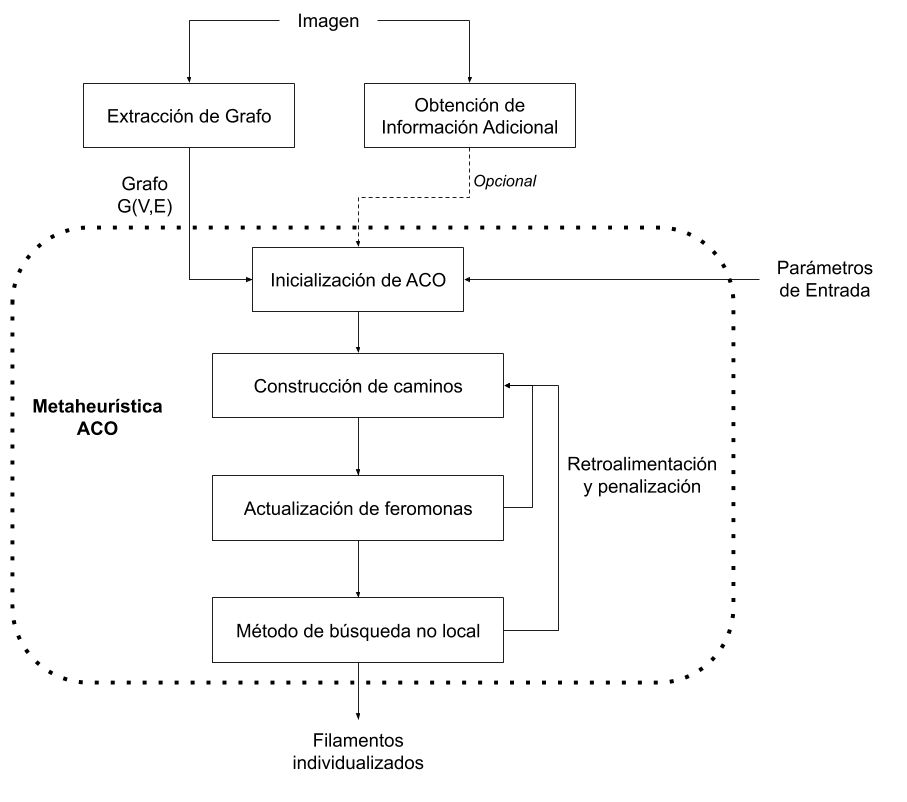
\includegraphics[height=2.8in]{Pictures/ACOdiagram.png}
\end{frame}

\note[itemize]{
    \item En particular,  el uso de ACO para la individualizaci\'on de filamentps se refleja en el diagrama, siendo ACO la parte central del algoritmo propuestp.
    \item Para preparar los datos de entrada para ACO, es necesario extraer desde una imagen un grafo que represente una red de filamentos, utilizando alguna herramienta externa.
    \item Adicionalmente es posible alimentar algunos par\'ametros de entrada de ACO en el algoritmo propuesto mediante informaci\'on conocida a priori del comportamiento de la c\'elula observada en la imagen de la que se extrae el grafo.
    \item Con lo anterior, el algoritmo propuesto entra al ciclo donde se encuentran las 3 etapas descrita en el algoritmo 1: La construcci\'on de caminos, la actualizaci\'on de feromonas y el m\'etodo de b\'usqueda no local
}

%\subsection{Problema de Satisfacci\'on de Restricciones}
% \begin{frame}{ACO aplicado como Problema de Satisfacci\'on de Restricciones (OE 1)}
%   \begin{columns}
%     \begin{column}{0.5\textwidth}
%         \begin{itemize}
%           \item $P = (S, \Omega, F)$
%           % esta definido por un conjunto discreto de variables
%           \item S:  Cjto. de soluciones, compuesto por variables discretas $X_{i}$, $i \in 1 \dotsc n$
%           %\item $S:\quad X = v_{i}^{j} \in D_{i} = \{v_{i}^{1} \dotsc  v_{i}^{|D_{i}|}\}$.
%           \item Sol. Candidata $s \in S$, y $s^{*}$ una soluci\'on \'optima
%           \item Cjto. de Restricciones $\Omega$
%           \item Funci\'on objetivo $F: S\rightarrow \mathbb R_{0}^{+}$
%           %\item  
          
%       \end{itemize}
%     \end{column}
%     \begin{column}{0.5\textwidth}
%       \begin{itemize}
%           \item $s$ es factible si satisface las restricciones de $\Omega$
%           % y se relacionan mediante 
%           \item Pueden existir m\'ultiples soluciones $s^{*}$
%           \item $S^{*}$ es el conjunto que engloba todas las soluciones \'optimas
%           \item $s^{*} \in S^{*} \subseteq S$
%       \end{itemize}
%     \end{column}
% \end{columns}
% \end{frame}





% \begin{frame}{Adaptaci\'on a Individualizaci\'on de Filamentos}
%     \begin{algorithm}[H]
%     \SetAlgoLined
%     \KwData{Variables $X_i \dotsc X_n$, dominios $D_1 \dotsc D_n$, Restricciones $\in \Omega$}
%     \KwResult{conjunto s\textquotesingle $ \subseteq S$ != $\emptyset$, si existen soluciones factibles}
%      Ajuste de Par\'ametros \& inicializaci\'on de feromonas \;
%      \While{Criterio de finalización no se cumple}{
%       Construcci\'on\_de\_soluci\'on\_de\_cada\_hormiga()\;
%       M\'etodo\_de\_b\'usqueda\_no\_local(); //Paso opcional\\
%       Actualizaci\'on\_de\_feromonas()\;
%      }
%      \caption{Algoritmo de un modelo COP adaptado a una metaheur\'istica ACO}\label{COP-ACO-Algo}
%     \end{algorithm}
% \end{frame}


\section{Algoritmo Propuesto}

\begin{frame}{ACO: Construcci\'on de Soluci\'on, Asignaci\'on de 1ra Arista (OE 1)}
    \begin{columns}
        \begin{column}{0.3\textwidth}
            \begin{itemize}
                \item Heur\'istica de Asignaci\'on Inicial: \begin{enumerate}
                    \item Arista con un nodo grado 1
                    \item Aristas en intersecciones
                    \item Arista aleatoria
                \end{enumerate}
                
            \end{itemize}
        \end{column}
        \begin{column}{0.7\textwidth}
            \centering
            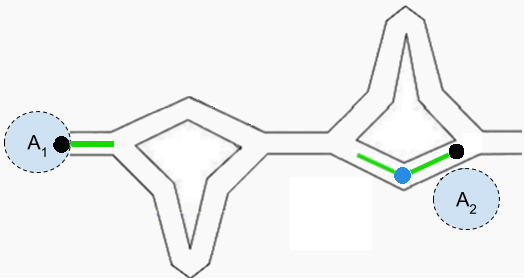
\includegraphics[scale=0.5]{Pictures/ant-initial-edge.png}
        \end{column}
    \end{columns}
\end{frame}

%\subsection{Construcci\'on de Soluciones}
% \begin{frame}{ACO: Construcci\'on de Soluci\'on (OE 1)}
% \centering
% 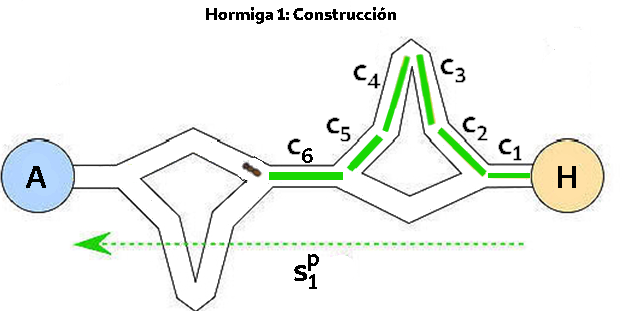
\includegraphics[scale=0.4]{Pictures/ACO-ant-Constr.png}
% \begin{itemize}
%     \item Influencia de feromonas $\tau$ y de una heur\'istica $\eta$ en la elecci\'on de Aristas/Componentes $c_i$ que respeten restricciones en $\Omega$
%     \item Aspecto aleatorio en la elecci\'on
% \end{itemize}
% \end{frame}

% \begin{frame}{ACO: Heur\'istica de Asignaci\'on Inicial}
% \begin{enumerate}
% \item Arista $a: (n_i,n_j)$ tal que $deg(n_i) = 1$ o $deg(n_j) = 1$ 
% %La arista a asignar debe tener al menos uno de sus nodos con grado 1, indicando que es el inicio o final de una parte del grafo.

% \item De no haber aristas disponibles con esas caracter\'isticas, se realiza una asignaci\'on inicial de una arista que cumpla con 2 criterios:
% \begin{itemize}
%     \item $a: (n_i,n_j)$ tal que $deg(n_i) >= 2$ o $deg(n_j) >= 2$ 
%     \item El \'angulo que forma la arista candidata a elegir, junto a otra arista a la que pertenece el nodo, debe pertenecer al rango $]\theta, Max\_Angle]$.
% \end{itemize}

% \item Una arista aleatoria que no pertenezca a una soluci\'on o camino evaluado como de buena calidad
% %. La calidad de un camino se presenta m\'as adelante en esta secci\'on.
% \end{enumerate}
% \end{frame}



\note[itemize]{
    \small
    \item la etapa de construcci\'on de una soluci\'on se compone de 2 partes: La asignaci\'on de la 1ra arista por donde la hormiga comenzar\'a su recorrido y de la elecci\'on de la siguiente arista a recorrer
    \item La asignaci\'on de la primera arista se realiza mediante una heru\'istica que consta de 3 criterios. El enfoque de estos criterios se centra en la exploraci\'on del espacio de b\'usqueda
    \item El primer criterio busca asignar aristas que esten en el borde del grafo, como la arista con uno de sus nodos en A1.
    
    \item De no existir m\'as aristas como las del 1er criterio, se buscan aristas que se encuentren en intersecciones, es decir que tengan uno de sus nodos con grado 2 o superior, y que el angulo que formen las aristas que comparten aquel nodo este en el rango intermedio definido previamente. Esto debido a que en varios tipos de filamentos hay casos en que los filamentos no nacen s\'olo del borde, sino tambi\'en a partir de otros filamentos. Un ejemplo de esto es una de las aristas que contiene al nodo en A2. 
    
    \item De no contar con aristas disponibles seg\'un los criterios previos, se elige una arista al azar, privilegiando las aristas que no son parte de un camino ya evaluado como una soluci\'on factible.
    
   \item Una vez que se le asigna una arista inicial a la hormiga, esta debe elegir que nuevas aristas irá agregando en su camino 

}


\begin{frame}{ACO: Construcci\'on de Soluci\'on (OE 1)}
    \begin{columns}
        \begin{column}{0.65\textwidth}
            \centering
            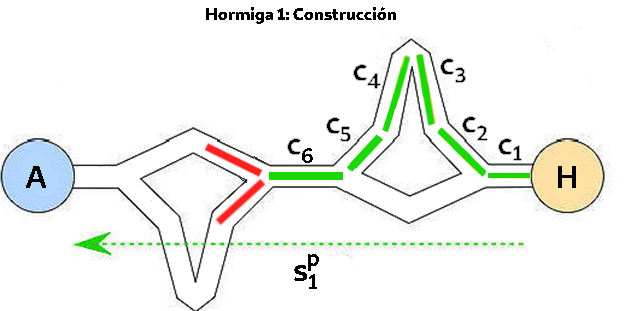
\includegraphics[scale=0.4]{Pictures/ACO-ant-Constr-choices.png}
        \end{column}
        \begin{column}{0.35\textwidth}
        \small
            \begin{equation}
            P(c_{i} | s^{P}) = \frac
            {\tau_{i} ~ \eta_{i}}
            {\sum\limits_{c_{j}\in N(s^p)}{\tau_{j} ~ \eta_{j} } } %, \forall c_{i} \in N(s^{P}).
            \label{eq:antProbabilities}
            \end{equation}
        \end{column}
    \end{columns}

    \begin{columns}
        \begin{column}{0.35\textwidth}
            \begin{itemize}
                \item Calidad $\sim$ Funci\'on Objetivo 
                %\item Calidad $s^{P}_1$ = $\sum \eta_{i}$
                \item Calidad $s_1$ = $\frac{1}{n}\sum \eta_{i} $
            \end{itemize}
        \end{column}
        \begin{column}{0.65\textwidth}
            \begin{itemize}%\fontsize{9pt}{10}\selectfont
                \item Calidad M\'inima $\geq \frac{Max\_Score}{2}$
                \item Buena Calidad: $Max\_Score$
                \item Calidad Intermedia: $[\frac{Max\_Score}{2}, Max\_Score[$
            \end{itemize}
        \end{column}
    \end{columns}
\end{frame}

\note[itemize]{
    \item Cada una de las posibles aristas vecinas a elegir tiene una probabilidad de ser elegida. Esta probabilidad se define seg\'un la ecuaci\'on a la derecha de la diapositiva y en esta influye la feromona $\tau$ y el valor de una heur\'istica $\eta$ asociada a cada arista.
    \item Esta heur\'istica entrega una puntuaci\'on asociada al \'angulo que forma la arista vecina con la última arista que fue agregada al camino o soluci\'on.
    
    \item a modo de ejemplo, las aristas en rojo representan las aristas vecina de C6, que fue la ùltima en ser añadida hasta ese punto al recorrido de la hormiga, teniendo cada una de las aristas rojas una probabilidad de ser elegida. 

    \item Una vez que la hormiga termina su recorrido, se evalua la soluci\'on mediante el promedio de los valores de eta. Esta evaluaci\'on corresponde a la funci\'on objetivo de la metaheur\'istica ACO y se puede separar en 3 rangos: 
    
    \item Las soluciones que no cumplen con una calidad m\'inima, que se desechan
    \item Las soluciones que se definen como de buena calidad, que son las que se eligen como soluciones candidatas
    \item y las soluciones que requieren de mayor evaluaci\'on dado que con los criterios aplicados durante la construcci\'on no pueden ser desechados ni aceptados.
    
    \item Luego, las soluciones de calidad intermedia y superior pasan a las siguientes etapas.
    
    \item NO LEER - Respira: se busca maximizar la funci\'on objetivo

}

%\subsection{M\'etodo de b\'usqueda no local}
\begin{frame}{B\'usqueda no local: l\'ogicas globales/centralizadas (OE 1)}
    
    \begin{columns}
        \begin{column}{0.4\textwidth}
            \begin{itemize}
                \item Eliminar soluciones candidatas que no aporten informaci\'on nueva
                \item Soluciones parcialmente repetidas
            \end{itemize}
        \end{column}
        \begin{column}{0.2\textwidth}
        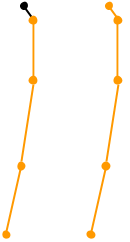
\includegraphics[scale=0.5]{Pictures/ant-segments-repetead-sol1.png}
        \end{column}
        \begin{column}{0.2\textwidth}
        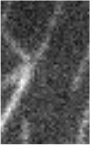
\includegraphics[scale=0.5]{Pictures/NoConsenso2.png}
        \end{column}
        \begin{column}{0.2\textwidth}
        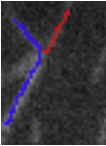
\includegraphics[scale=0.5]{Pictures/NoConsenso3.png}
        \vspace{0.5cm}
        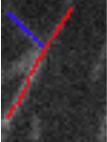
\includegraphics[scale=0.5]{Pictures/NoConsenso4.png}
        \end{column}
    \end{columns}
\end{frame}

\note[itemize]{
\small
    \item Una de las etapas siguientes corresponde a la b\'usqueda no local, la que se basa en l\'ogicas globales o centralizadas, a diferencia de la construcci\'on de soluciones de cada hormiga que es miope.
    %\item La b\'usqueda de soluciones de cada hormiga puede llevar a que dos o m\'as hormigas encuentren soluciones que son muy similares, repitiendo informaci\'on.
    \item Esta etapa busca eliminar soluciones duplicadas o muy similares, privilegiando las soluciones que contengan dentro de si a otras. A modo de ejemplo, en naranjo se muestran dos soluciones similares, siendo la soluci\'on de la derecha levemente m\'as larga.
    \item Se elige la soluci\'on m\'as larga para evitar ambiguedades y que en caso de error, la soluci\'on indicada como un filamento sea igual o m\'as extensa en vez de ser corta con respecto a lo que pueda indicar un experto
    \item Este an\'alisis es similar al que puede suceder entre 2 expertos que ante la misma imagen identifiquen distintos filamentos, como se ejemplifica con las im\'agenes de la derecha.
    
}

% \begin{frame}{ACO: Actualizaci\'on de Feromonas (OE 1)}
% \centering
% 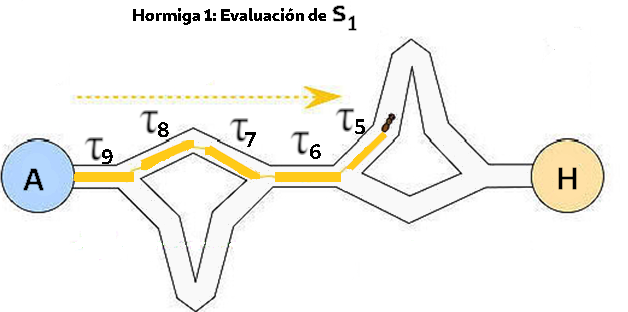
\includegraphics[scale=0.4]{Pictures/ACO-ant-ferom.png}
% \begin{itemize}
%     
% \end{itemize}
% \end{frame}


%\subsection{Anti-feromonas}
\begin{frame}{ACO: Actualizaci\'on de feronomas, uso de Anti-feromonas SAP (OE 1)}
    \centering
    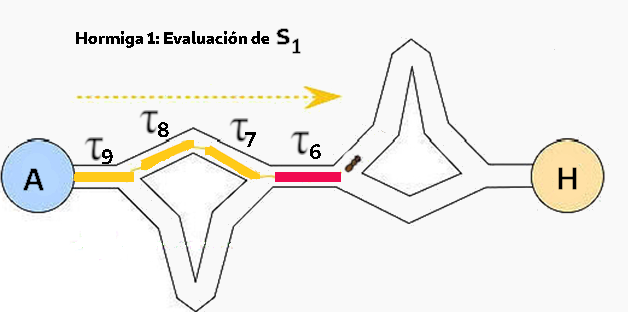
\includegraphics[scale=0.4]{Pictures/ACO-ant-ferom-penalize.png}
    \begin{columns}
        \begin{column}{0.5\textwidth}
            \begin{itemize}
            \small
                \item Evaluaci\'on de factiblidad de soluciones candidatas $s \in S$
                \item Feronomonas: premiar los caminos de buena calidad para lograr onvergencia sobre un camino \'optimo
                
            \end{itemize}
        \end{column}
        \begin{column}{0.5\textwidth}
            \begin{itemize}
            \small
                \item Cambio: $\tau_0 \longrightarrow \gamma$
                \item $\gamma$ es un factor penaliza los caminos de mala calidad
                \item 2 penalizaciones $\longrightarrow \tau_i = 0$ 
            \end{itemize}
        \end{column}
    \end{columns}
    
\end{frame}

\note[itemize]{
    \item la \'ultima etapa a mencionar corresponde a la actualizaci\'on de feromonas. Al finalizar el recorrido de una hormiga, es necesario actualizar el valor de la feromonas. En el caso de una metaheur\'istica ACO tradicional, se aumenta el valor de tau para cada arista que pertenece a un camino de buena calidad.
    \item Sin embargo, ese enfoque privilegia la convergencia sobre un sola soluci\'on, y a su vez puede ocasionar la perdida de soluciones factibles.
    \item Para evitar eso, se propone el uso de Anti-feromonas, cuyo objetivo es acotar el espacio de b\'usqueda mediante la penalizaci\'on de los caminos o soluciones de mala o baja calidad.
    \item As\'i, el valor de tau que influye en la probabilidad de elecci\'on de una arista disminuye, pudiendo llegar a cero, lo que ocasiona que esa arista no pueda ser elegida por ninguna hormiga que aun este construyendo una soluci\'on.
}

\begin{frame}{Problema de Anti-feromonas SAP (OE 1)}
\centering
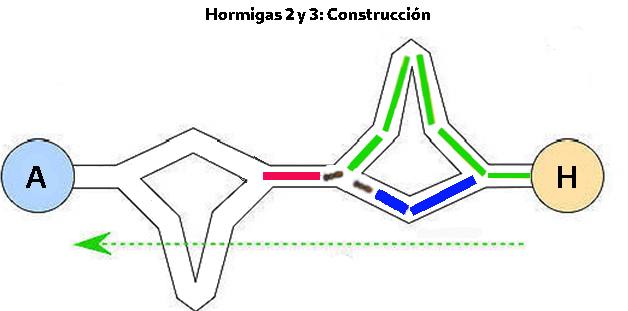
\includegraphics[scale=0.4]{Pictures/ACO-ant-constr-penalize.png}
    \begin{itemize}
        \item Problema: penalizaci\'on puede ocasionar perdida de soluciones factibles
        \item Propuesta: Relacionar penalizaci\'on de $\tau_i$ con $c_i \in s^P$
    \end{itemize}
\end{frame}

\note[itemize]{
    \item Sin embargo, el cambio de feromonas a anti-feromonas no soluciona el problema que se puede originar al focalizar la penalizaci\'on solo en las aristas.
    
    \item Una arista con un tau penalizado por pertenecer a uno o más caminos de mala calidad, puede bloquear otros caminos, dado que el valor de tau no guarda relación con las otras aristas que conforman el camino de mala calidad que caus\'o la penalización. Así, las soluciones que pudiesen pasar por esa arista se ven limitadas.
    
    \item A modo de ejemplo, el camino verde que es de mala calidad origina una penalizaci\'on sobre la arista en rojo. Luego, el camino azul, que puede construir una soluci\'on de buena calidad si incorpora la arista en rojo, se ve bloqueado, ya que la arista roja tiene una penalizaci\'on que hace menos probable o derechamente imposible su elecci\'on.
    
    

}

\begin{frame}{Anti-feromonas SAP dependientes del camino previo (OE 1)}
    \centering
    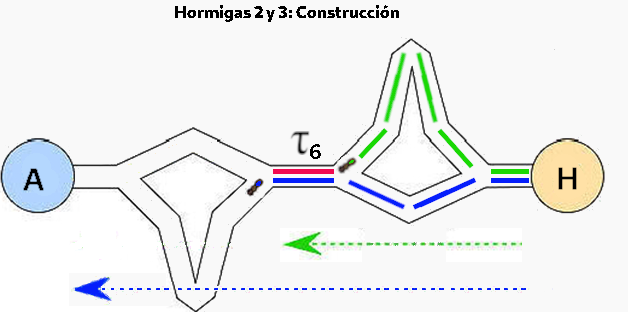
\includegraphics[scale=0.51]{Pictures/ACO-ant-ferom-penalize-seg.png}
\end{frame}

\note[itemize]{
    \item Por ende, se propone un cambio para que la penalizaci\'on de una arista guarde relaci\'on con con el conjunto de aristas que la preceden en el camino
    \item As\'i, solo hormigas que repitan parcial o totalmente l camino verde no podran elegir la arista en rojo, mientras que hormigas que provengan de otro recorrido, como la hormiga del camino azul no se ver\'an afectadas, evitando la perdida de soluciones.
    
    \item El conjunto de aristas predecesoras se denomina segmento.

}

% \begin{frame}{Anti-feromonas sobre un segmento de una sola arista (OE 1)}
%     \centering
%     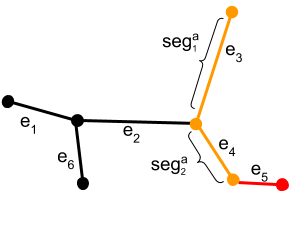
\includegraphics[height=2in]{Pictures/ant_segments_complex_case_B2.png}
%     \hspace{0.1cm}
%     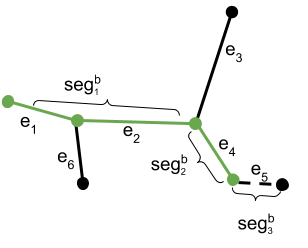
\includegraphics[height=2in]{Pictures/ant_segments_complex_case_B_blocked.png}
% \begin{itemize}
%     \item Segmentos de una sola arista ocasionan mismo problema que se intenta resolver
% \end{itemize}
% \end{frame}

% \begin{frame}{Anti-feromonas sobre un segmento (OE 1)}
% \centering
%     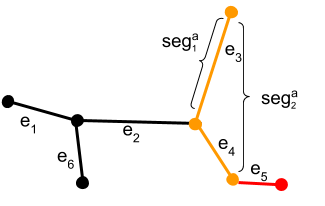
\includegraphics[scale=0.5]{Pictures/ant_segments_complex_case_B2_extended.png}
%     \begin{itemize}
%         \item Se extiende el segmento unitario con el segmento que lo precede
%     \end{itemize}
% \end{frame}

%\subsection{Criterios para la Actualizaci\'on de Anti-feromonas}
\begin{frame}{Criterios de Anti-feromonas sobre soluciones de calidad intermedia (OE 1)}
\begin{enumerate}
    
    \item Curvatura de una soluci\'on
    \item Magnitud de desplazamiento entre segmentos
    \item Criterio espec\'ifico para neuronas
\end{enumerate}
\end{frame}

\note[itemize]{
    \item Los 2 primeros criterios se relacionan a la rigidez que presenta un filamento, el que varía dependiendo de la estructura observada. 
}

\begin{frame}{Curvatura de una soluci\'on (OE 1)}
\centering
    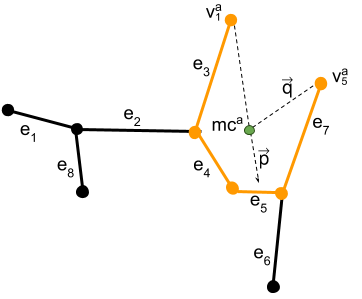
\includegraphics[scale=0.5]{Pictures/ant_curvature_case.png}
    \begin{itemize}
        \item El \'angulo entre la proyecci\'on de $\Vec{p}$ y $\Vec{q}$ debe ser menor a $\theta \times Max\_Axial\_Displacement$ para no descartar la soluci\'on.
    \end{itemize}
\end{frame}

\note[itemize]{
\item una soluci\'on como la destacada en color naranja se puede calificar como una soluci\'on infactible debido a su pronunciada curvatura, lo que no es normal de observar en los filamentos. 
\item As\'i, el c\'alculo de esta curvatura corresponde al \'angulo formado entre el vector q y la proyecci\'on del vector p. Este \'angulo debe respetar el umbral que define la multiplicaci\'on de los par\'ametros theta y Max axial displacement
}

\begin{frame}{Magnitud de desplazamiento entre segmentos (OE 1)}
    \centering
    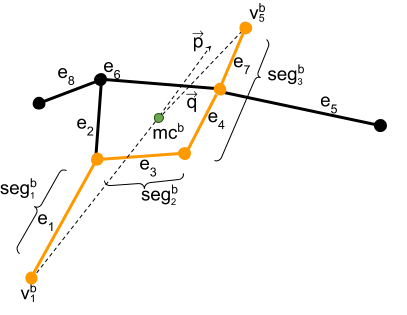
\includegraphics[height=2in]{Pictures/ant_segmentMagnitude_case.png}
    \hspace{0.2cm}
    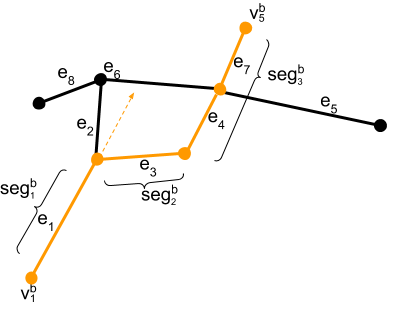
\includegraphics[height=2in]{Pictures/ant_segmentMagnitude_case_2.png}
    \begin{itemize}
        %\item El criterio de curvatura puede no ser suficiente por si mismo
        \item Comportamiento esperado de la rigidez permite descartar soluciones con cambios demasiado pronunciados entre sus segmentos
    \end{itemize}
\end{frame}

\note[itemize]{
\item 
}

%%\subsection{Extracci\'on de informaci\'on para individualizar filamentos}
\begin{frame}{Criterio espec\'ifico para neuronas (OE 1)}
    \begin{itemize}
        \item Se debe validar que los filamentos de una neurona parten del {\bf soma}
        \item  Extracci\'on de informaci\'on: caracter\'isticas geom\'etricas, topol\'ogicas y espaciales
    \end{itemize}
    \begin{columns}
        \begin{column}{0.55\textwidth}
        \centering
        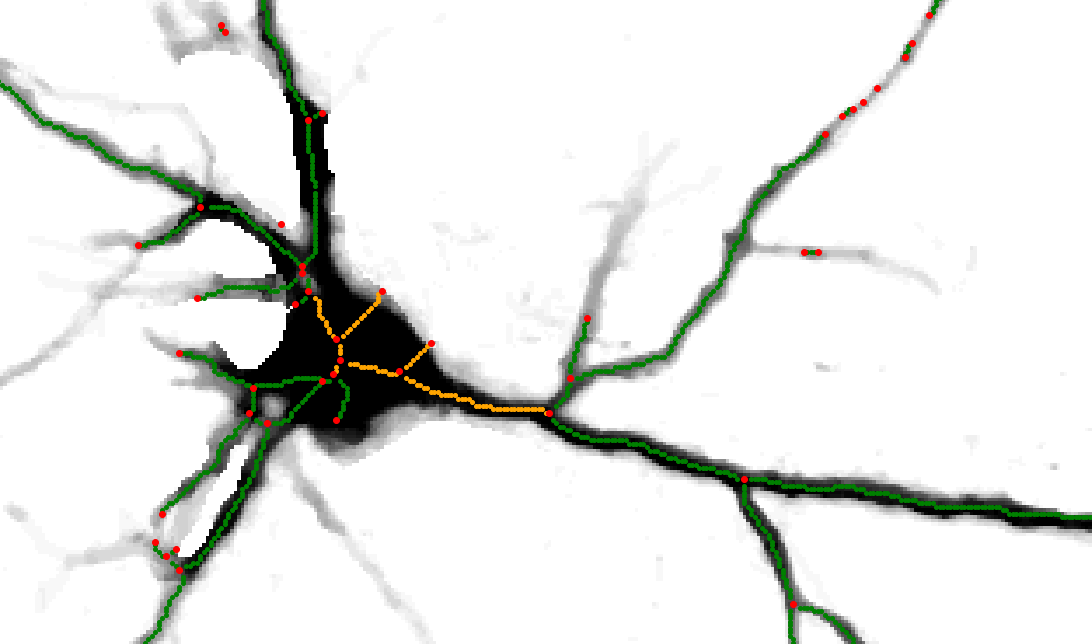
\includegraphics[height=1.7in]{Pictures/Porta183-somaEdges-example2.png}
        \end{column}
        \begin{column}{0.45\textwidth}
            \begin{equation}
                \tau_{ij} \leftarrow
                    \begin{cases}
                     \tau_{ij} \cdot \gamma \text{ si } deg(v^{a}_{n}) = 1,  \\[3ex]
                    
                    \text{0 si } \tau_{ij} \leq 0.25, \\[3ex]
                    \tau_{ij} \quad \text{en otro caso}.
                    \end{cases}
            \end{equation}
        \end{column}
    \end{columns}
    
\end{frame}

% \begin{frame}{Extracci\'on de informaci\'on para individualizar filamentos}
%      \begin{figure*}[h!]
%     \centering
%     \begin{subfigure}[t]{0.48\textwidth}
%         \centering
%         %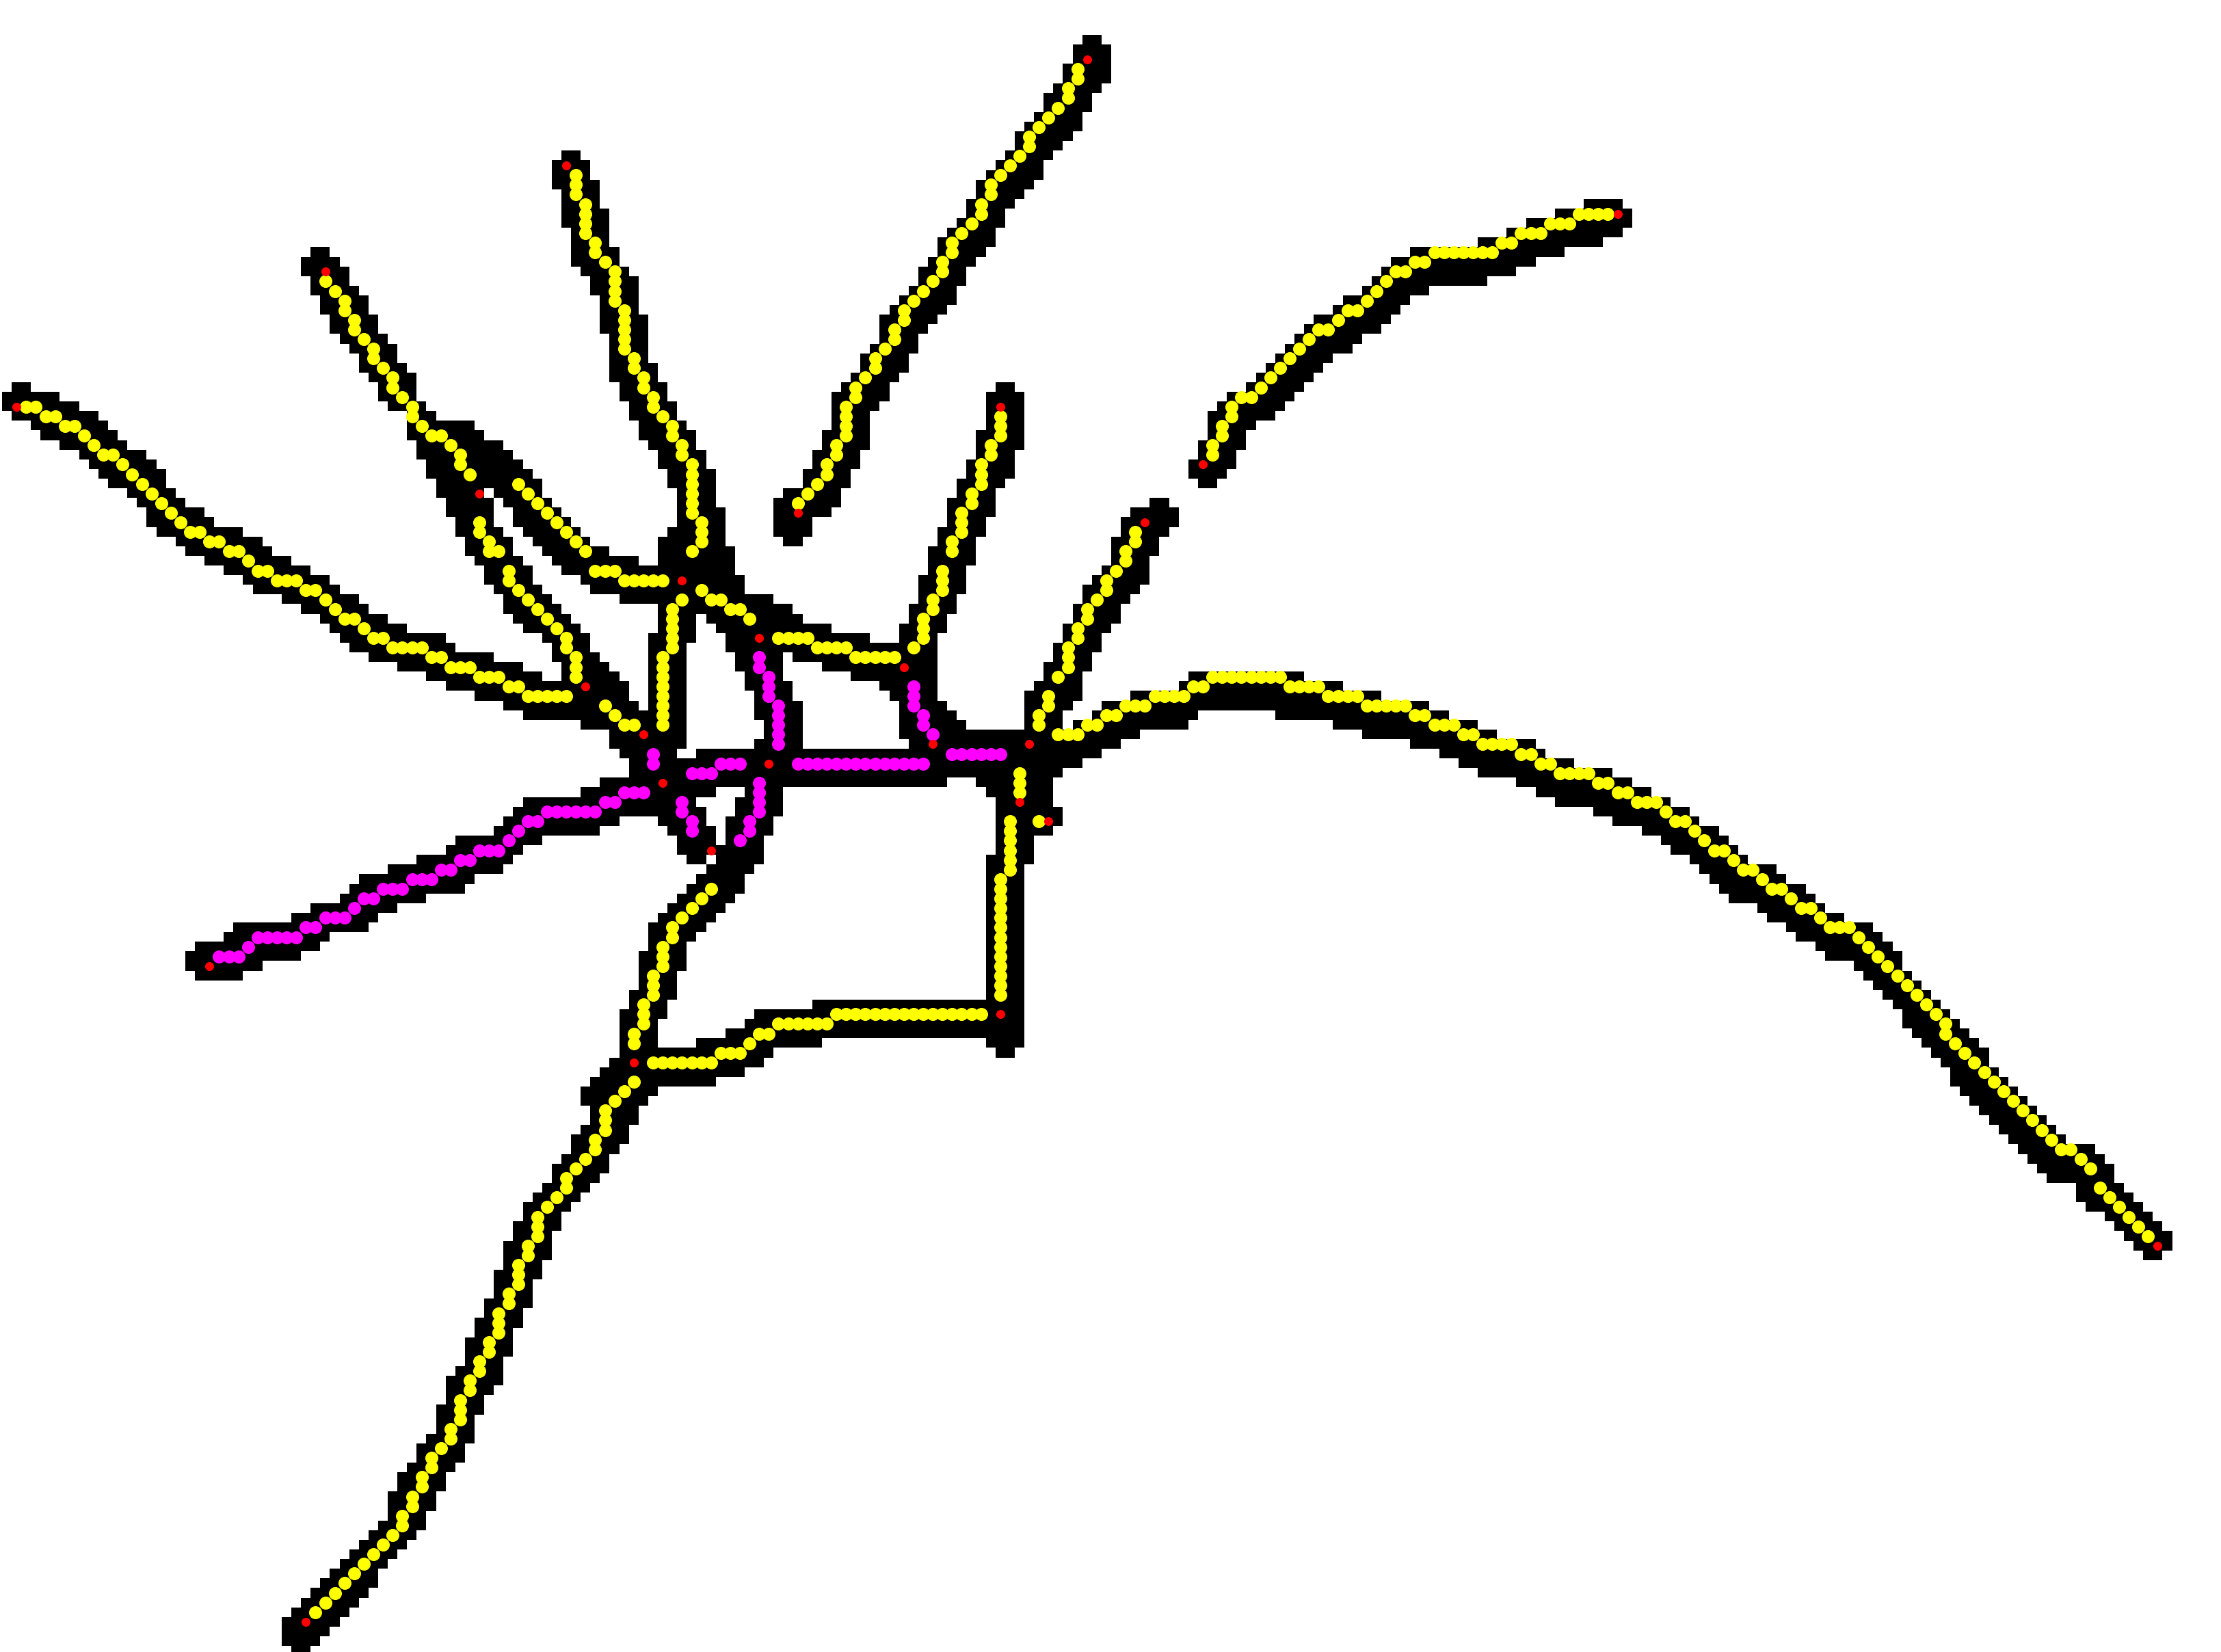
\includegraphics[height=1.5in]{Pictures/50-ROIs-Spinning-Marchantia-somaEdges.png}
%     \end{subfigure}%
%     ~ \hspace{0.1cm}
%     \begin{subfigure}[t]{0.48\textwidth}
%     \centering
%         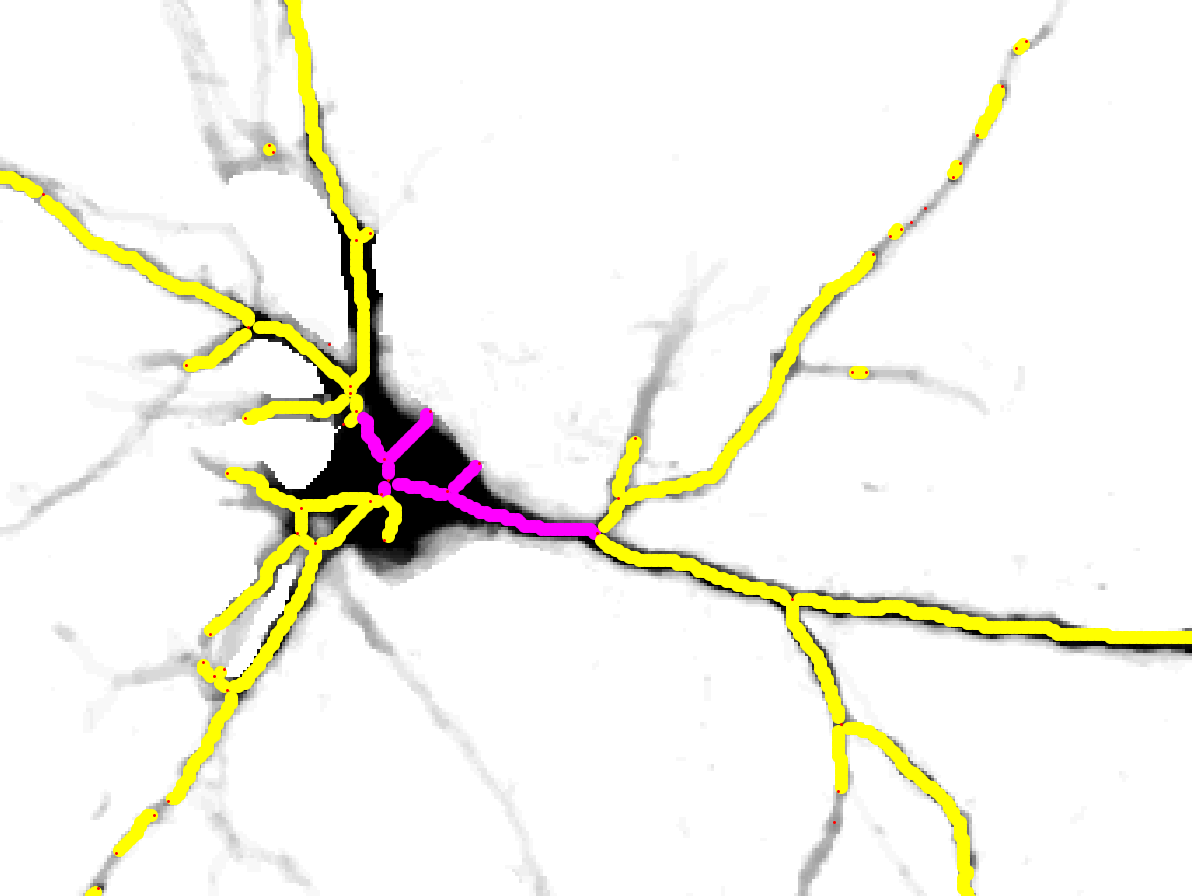
\includegraphics[height=1.5in]{Pictures/Porta18-3a1-somaEdges.png}
%     \end{subfigure}
%     \end{figure*}
%     \begin{itemize}
%         \item Caracter\'isticas geom\'etricas, topol\'ogicas y espaciales
%     \end{itemize}
% \end{frame}